\documentclass[UTF8]{ctexart}

\usepackage{subfiles}  

%下面的语句, 引入你的头部设置文件
\usepackage{C:/phpStorm_proj/02_myself_ID_EGO/+100_latex_all_math_sel/myPreamble} 
%必须是绝对路径,才能让各个tex在单独编译时使用到

\title{文件名}


%---------------------------------


\begin{document}
	\tableofcontents % 生成目录
	\date{} % 若不写这句, 则默认也会渲染出日期, 所以我们要手动赋空值
	\maketitle  %这行代码, 让你前面的 title, author, date生效
	
	
	\part{累积函数 Cumulative Distribution Function (CDF)}
	
	
	\section{累积函数 $ \boxed{	F\left( x \right) =P\left\{ X\leq x \right\} =\sum_{x_k\leq x}^{}{p_k}}$  ← 是对``概率函数"值的累加结果}
	
	
	对于随机变量, 我们通常关心的, 并不是它取某个值的概率(即我们并不关心它的分布律), 而是更关心它落在某个区间内的概率.  \\
	比如, 对某考试, 我们更关心的是``不及格的总人数", 和比如 ``分数≥80分 的总人数". \\
	
	
	累积函数 Cumulative Distribution Function (CDF) ← 是对``概率函数"值的累加结果 . 即对``概率密度函数"的积分.  \\
	
	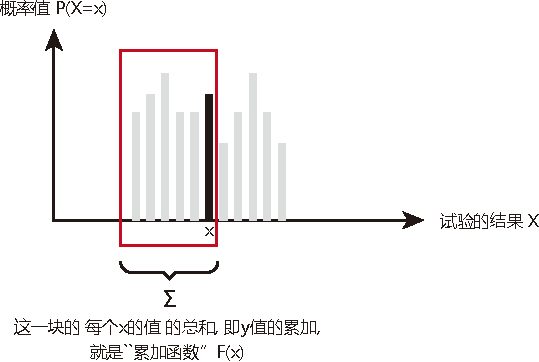
\includegraphics[width=0.7\textwidth]{/0118.pdf} \\
	
	
	在这些个区间段所占的概率值, 就是用``累加函数"(又叫``分布函数")来表示的. 即: \\
	$ (\text{随机变量}X\leq \text{自变量}x)=\underset{\text{累加函数}}{\underbrace{F(x)}}
	$ ← 它表示随机变量X 落在 (-∞, x] 这段区间上的概率. \\
	
	$\boxed{
		\text{累加函数} F\left( x \right) =P\left\{ X\leq x \right\} =\sum_{x_k\leq x}^{}{p_k}
	}$ \\
	
	累加函数 F(x) 就是 ``X取≤x 的所有值$x_k$" 的概率之和. \\
	P(X≤x) 即``X的取值不超过x" 的概率. 这里P后面写()或\{\}都行, 意思是一样的. \\
	
	
	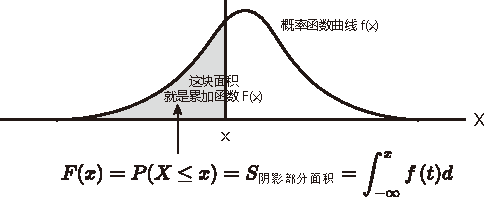
\includegraphics[width=0.7\textwidth]{/0125.pdf} \\
	
	
	
	
	下图, 左边两张是``概率函数", 右边两张就是``累加函数 CDF". \\
	
	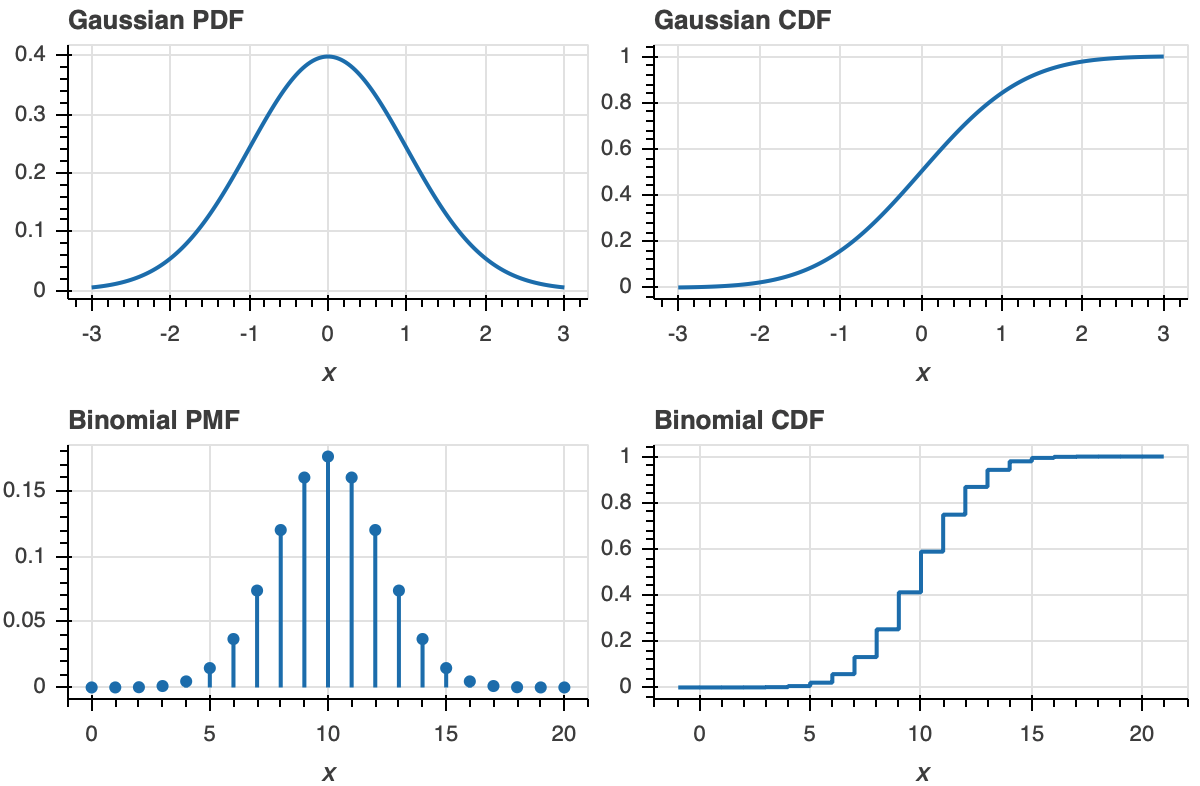
\includegraphics[width=1\textwidth]{/0117.png} \\
	
	
	
	
	
	\begin{myEnvSample}
		下面的图, 左边是``概率函数", 右边是``累加函数". \\
		
		离散型数据的: \\
		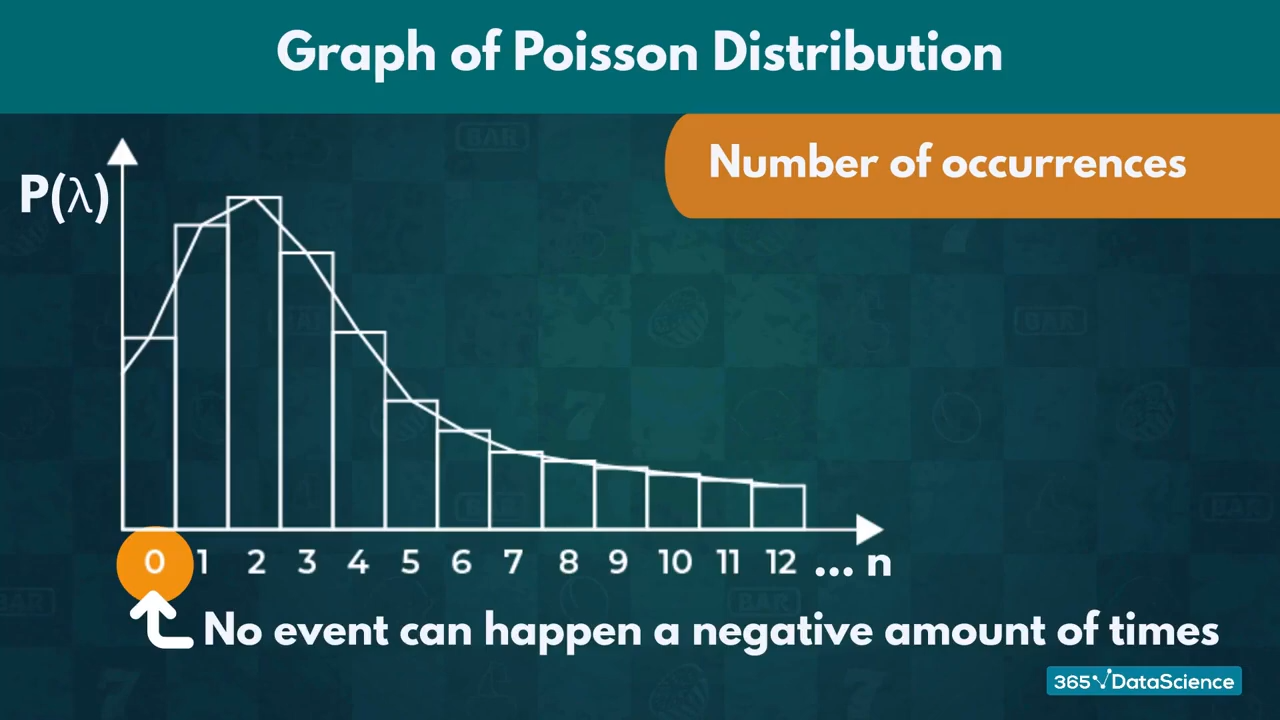
\includegraphics[width=0.8\textwidth]{/0122.png} \\
		
		连续型数据的: \\
		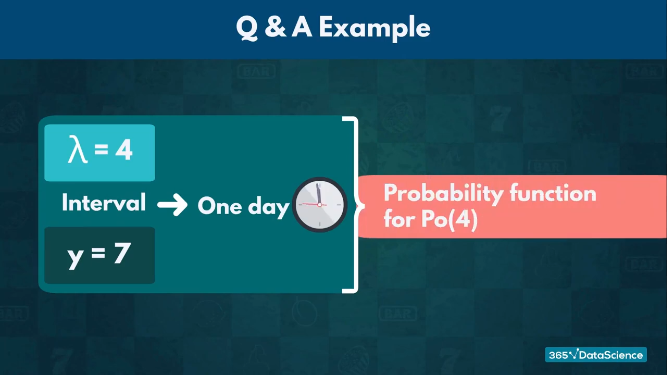
\includegraphics[width=0.8\textwidth]{/0123.png} 
	\end{myEnvSample} 
	
	
	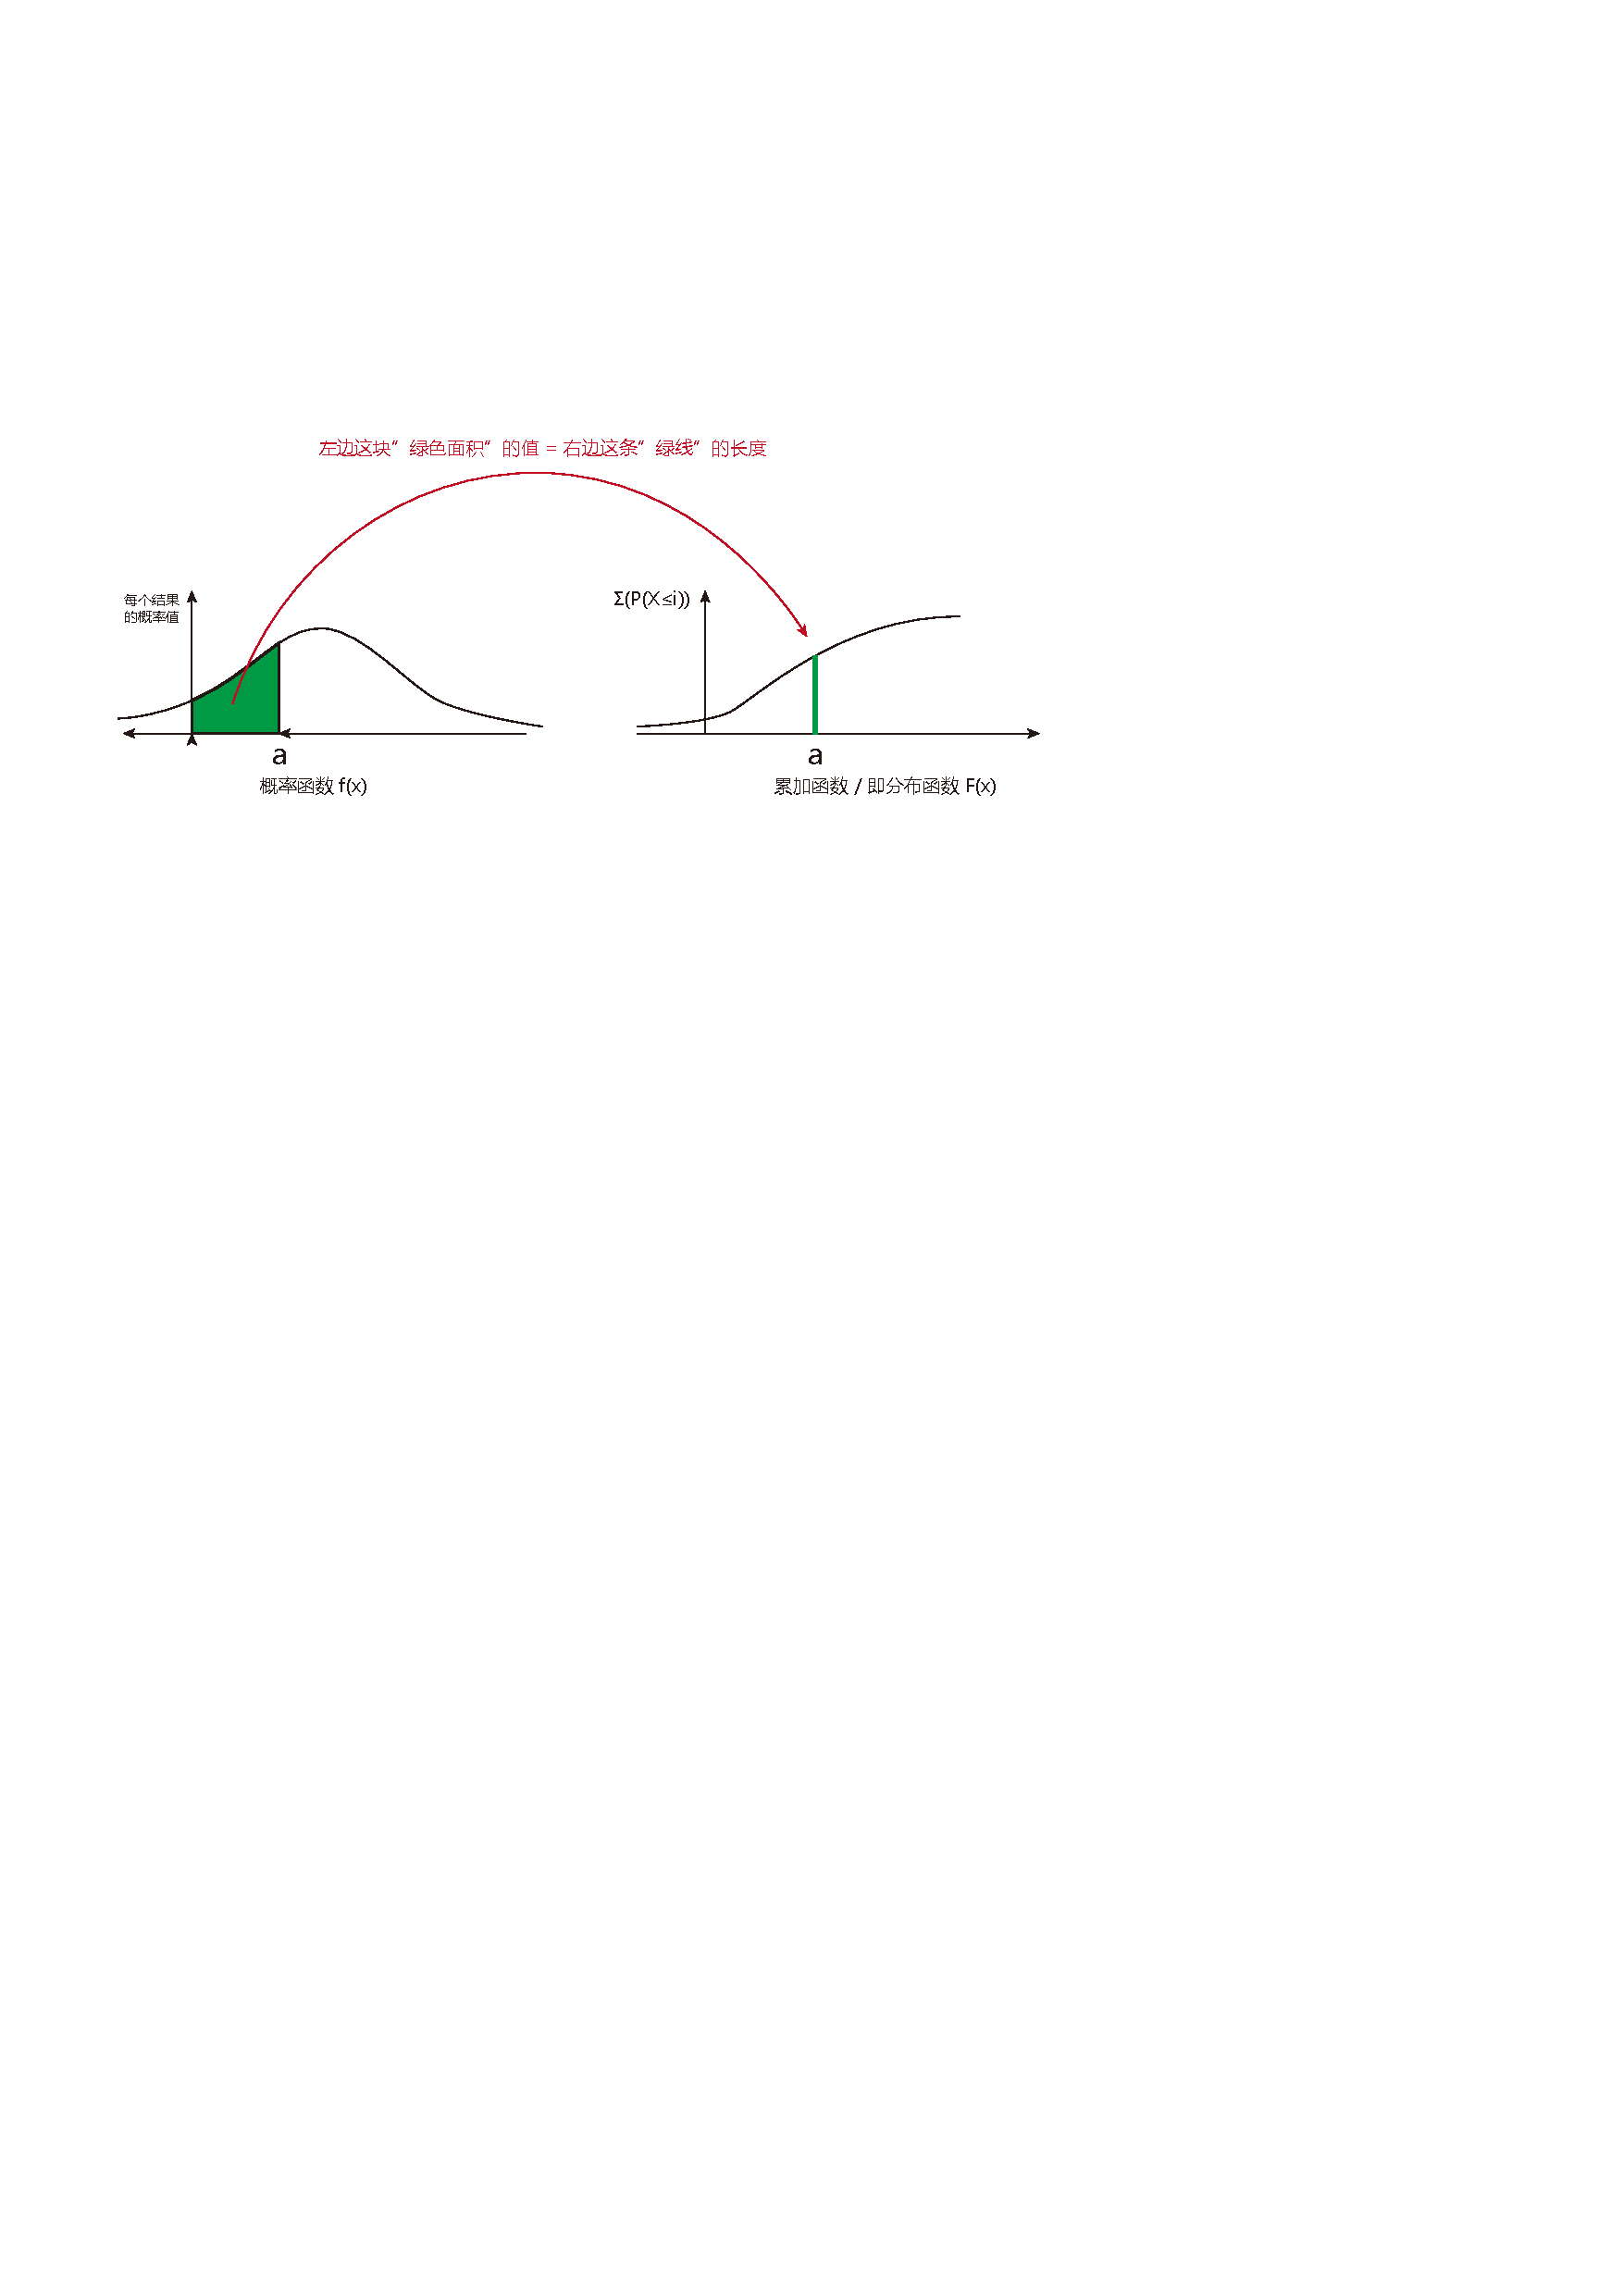
\includegraphics[width=0.8\textwidth]{/0128.pdf} \\
	
	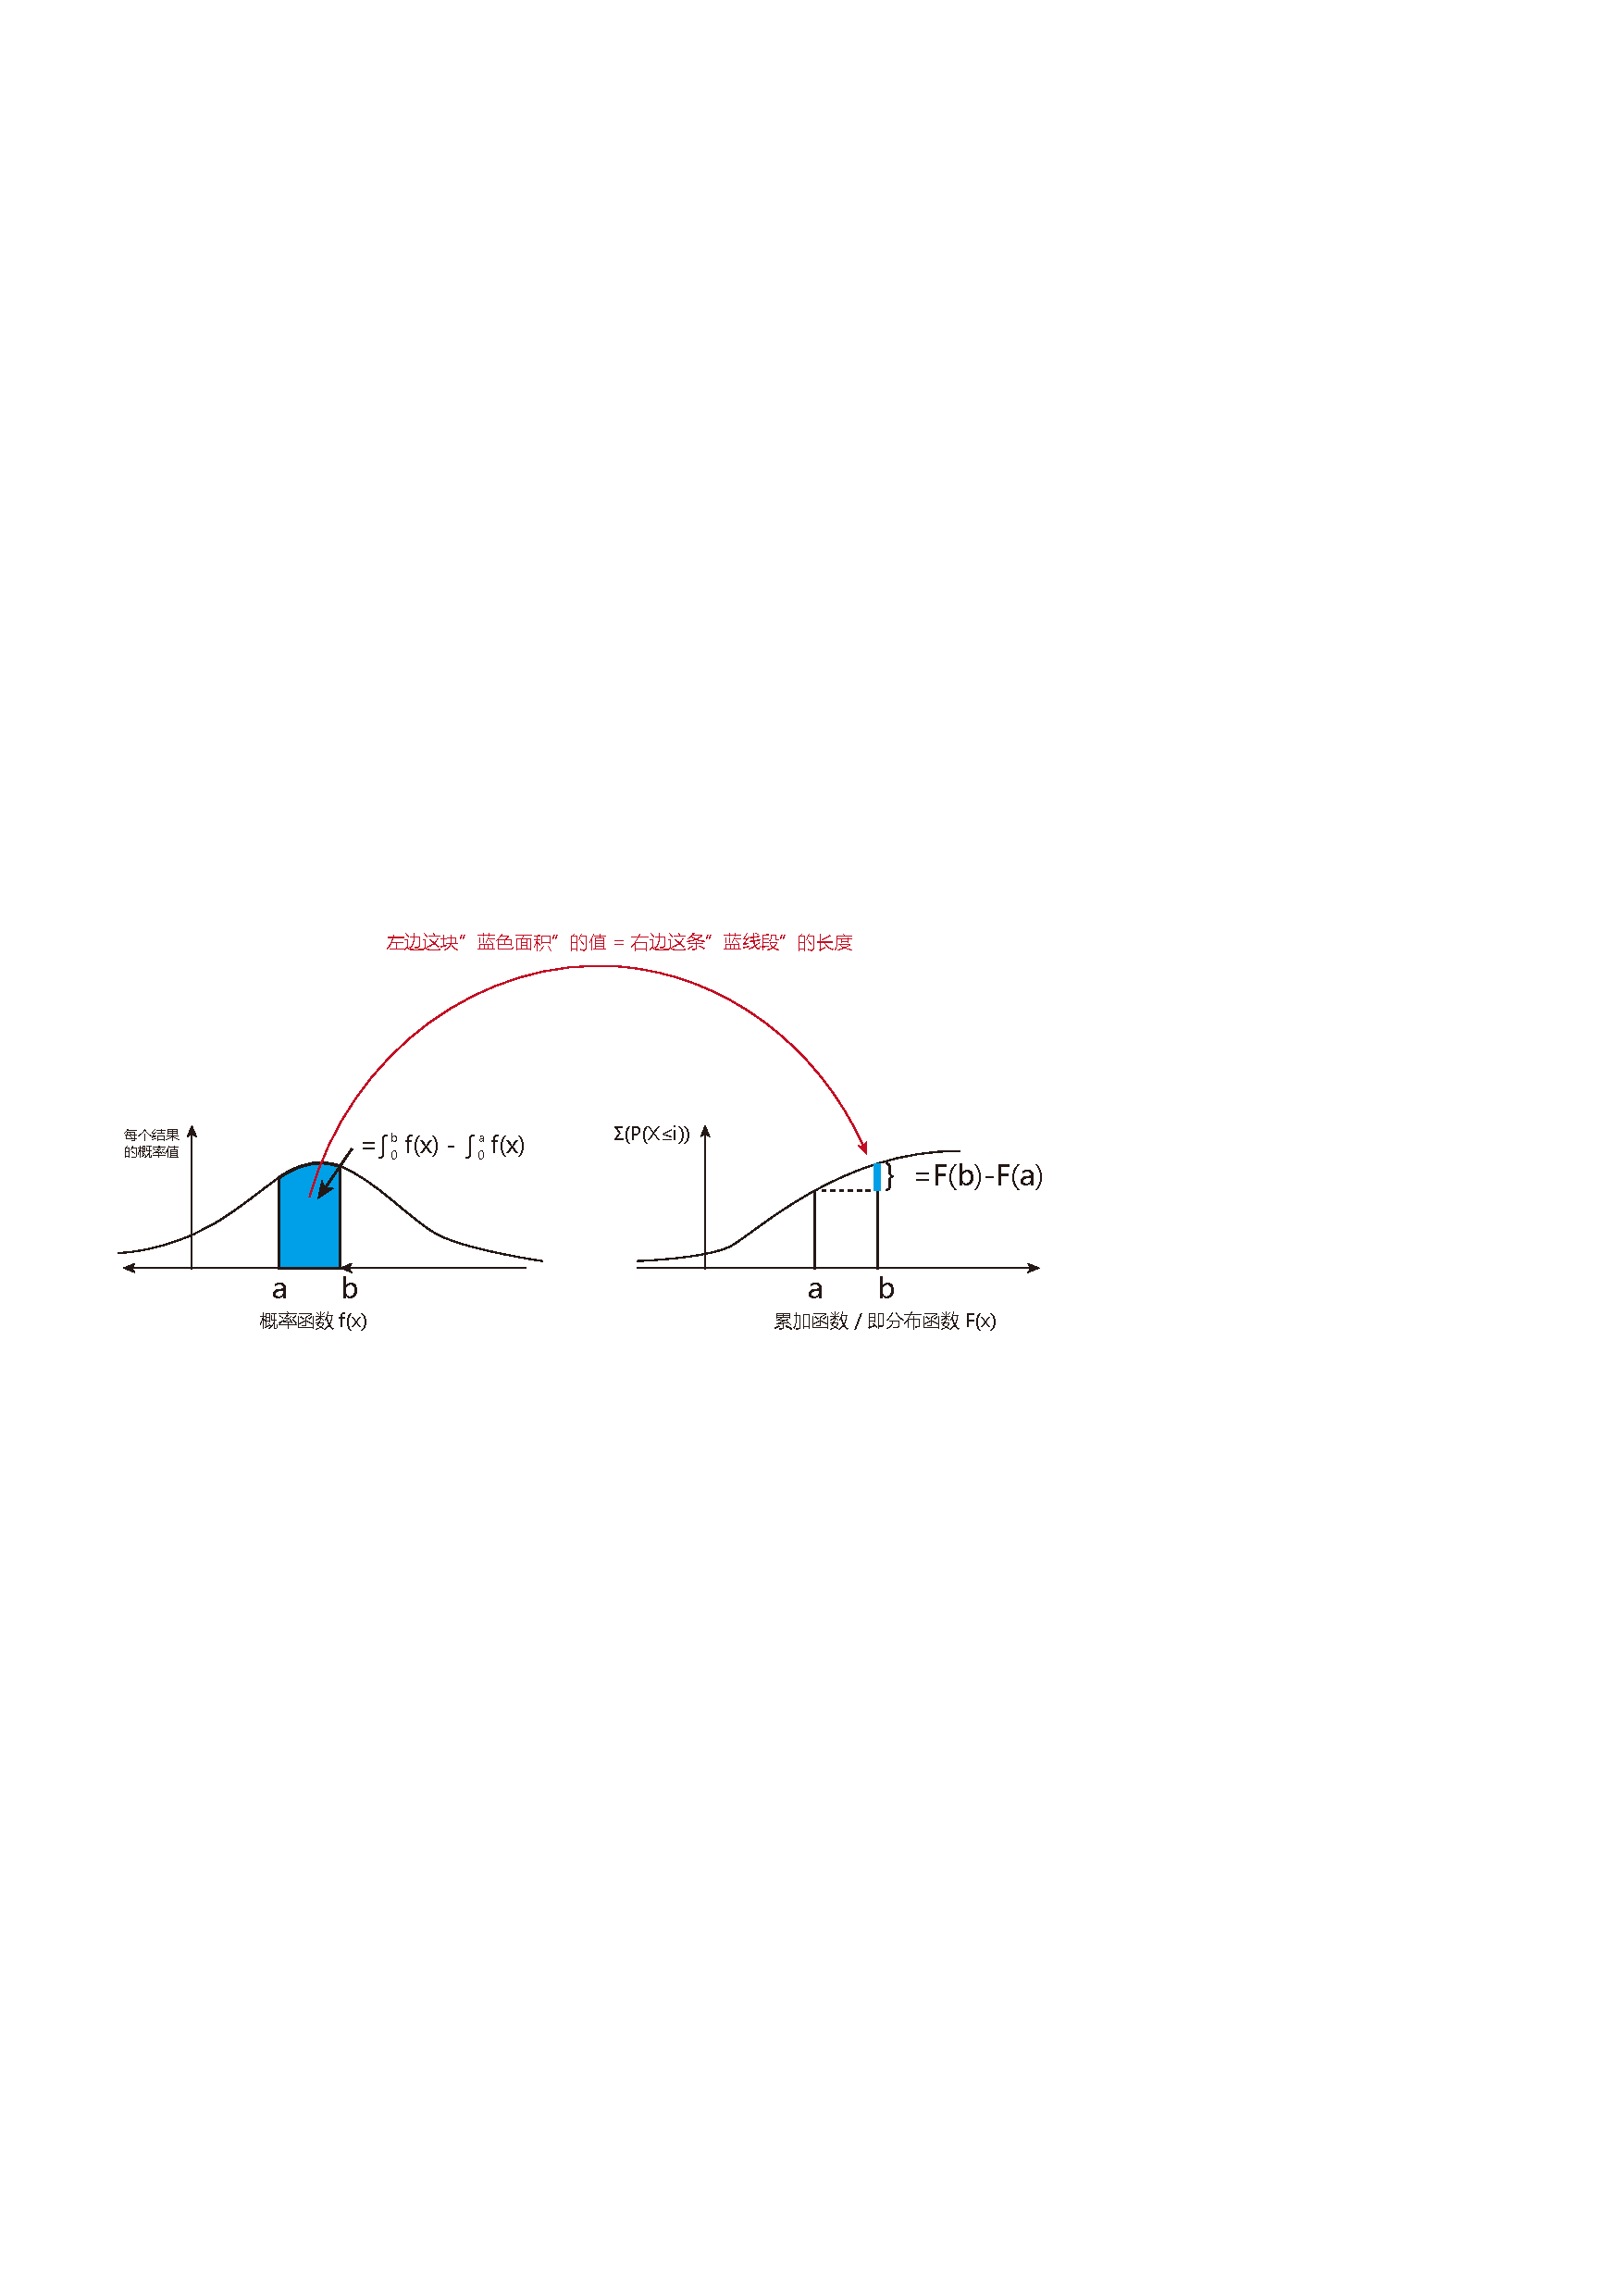
\includegraphics[width=0.8\textwidth]{/0129.pdf} \\
	
	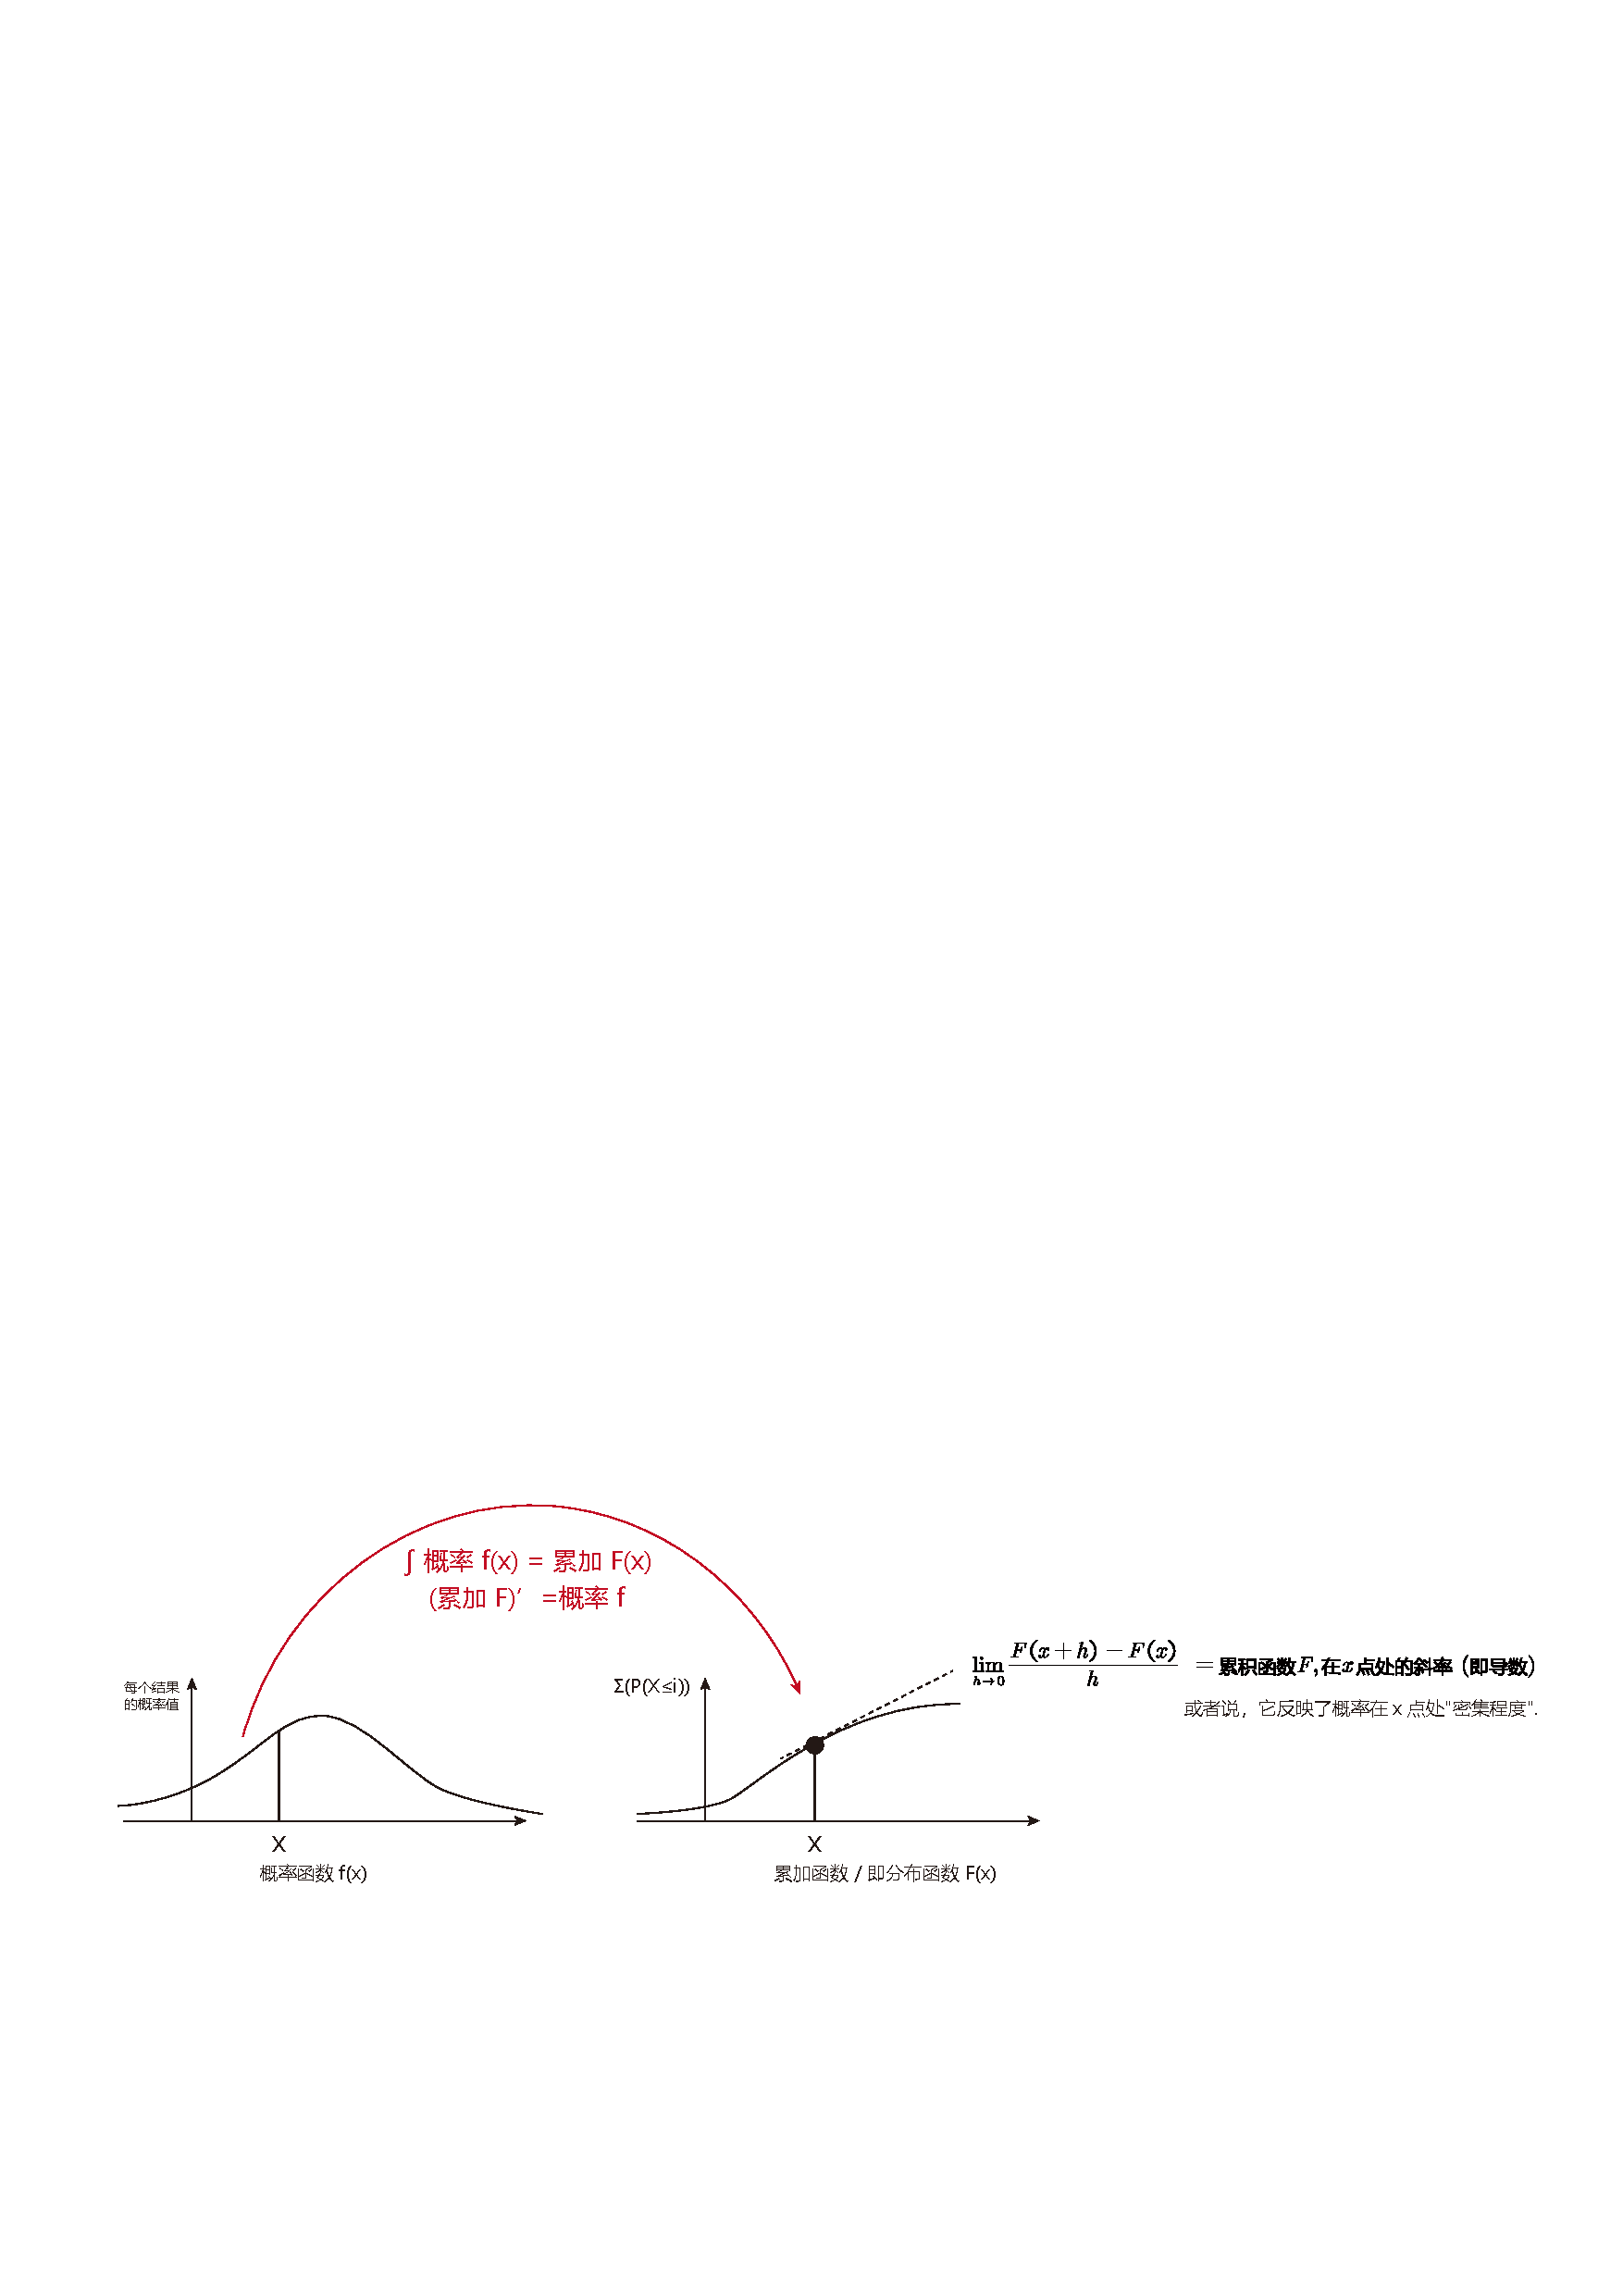
\includegraphics[width=1\textwidth]{/0130.pdf} \\
	
	
	~\\
	\hrule
	~\\
	
	
	\section{ ★  累加函数的计算公式}
	
	\begin{tabular}{|p{0.5\textwidth}|p{0.5\textwidth}|}
		\hline
		累加函数 $F(x)=P{X \leq x}$ 的公式有 & 图中: 蓝-绿=橙 \\
		\hline
		(1) $P\{X \leq a\} = F(a)$ &  \\ \hline
		(2)  $P\{X < a\} = F(a-0)$ ← 其中的 F(a-0) : 就是从左边逼近a, 不包括a点. 所以是``左极限". 就是(-∞,a)这段区间的概率之和, 不包括a点上的概率.  &  \\ \hline
		(3) $P\{X > a\} = 1- P\{X \leq a\} = 1- F(a)$ &  \\ \hline
		(4) $P\{X \geq a\} = 1- F(a-0)$ & 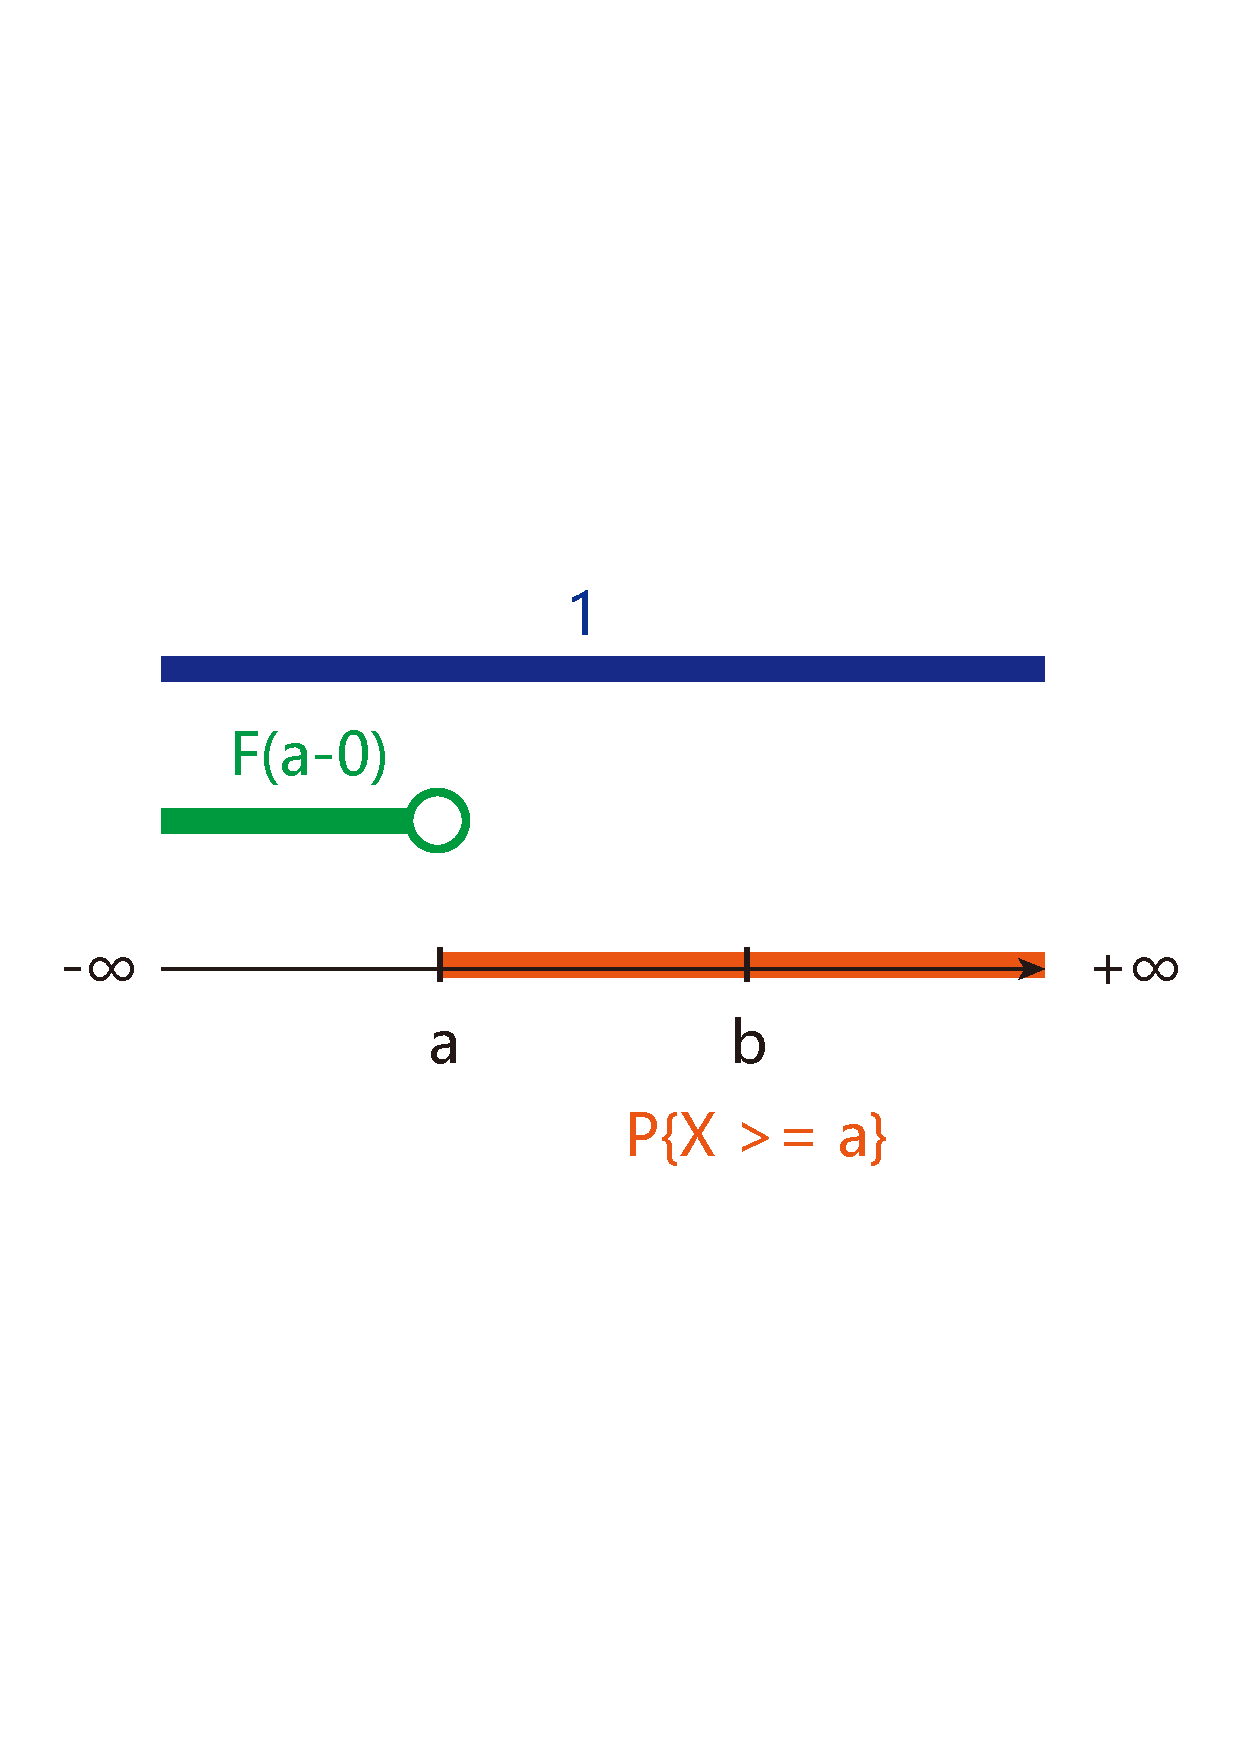
\includegraphics[width=0.4\textwidth]{/0132.pdf}
		\\ \hline
		(5) $P\{X=a\} = F(a) - F(a-0)$ &  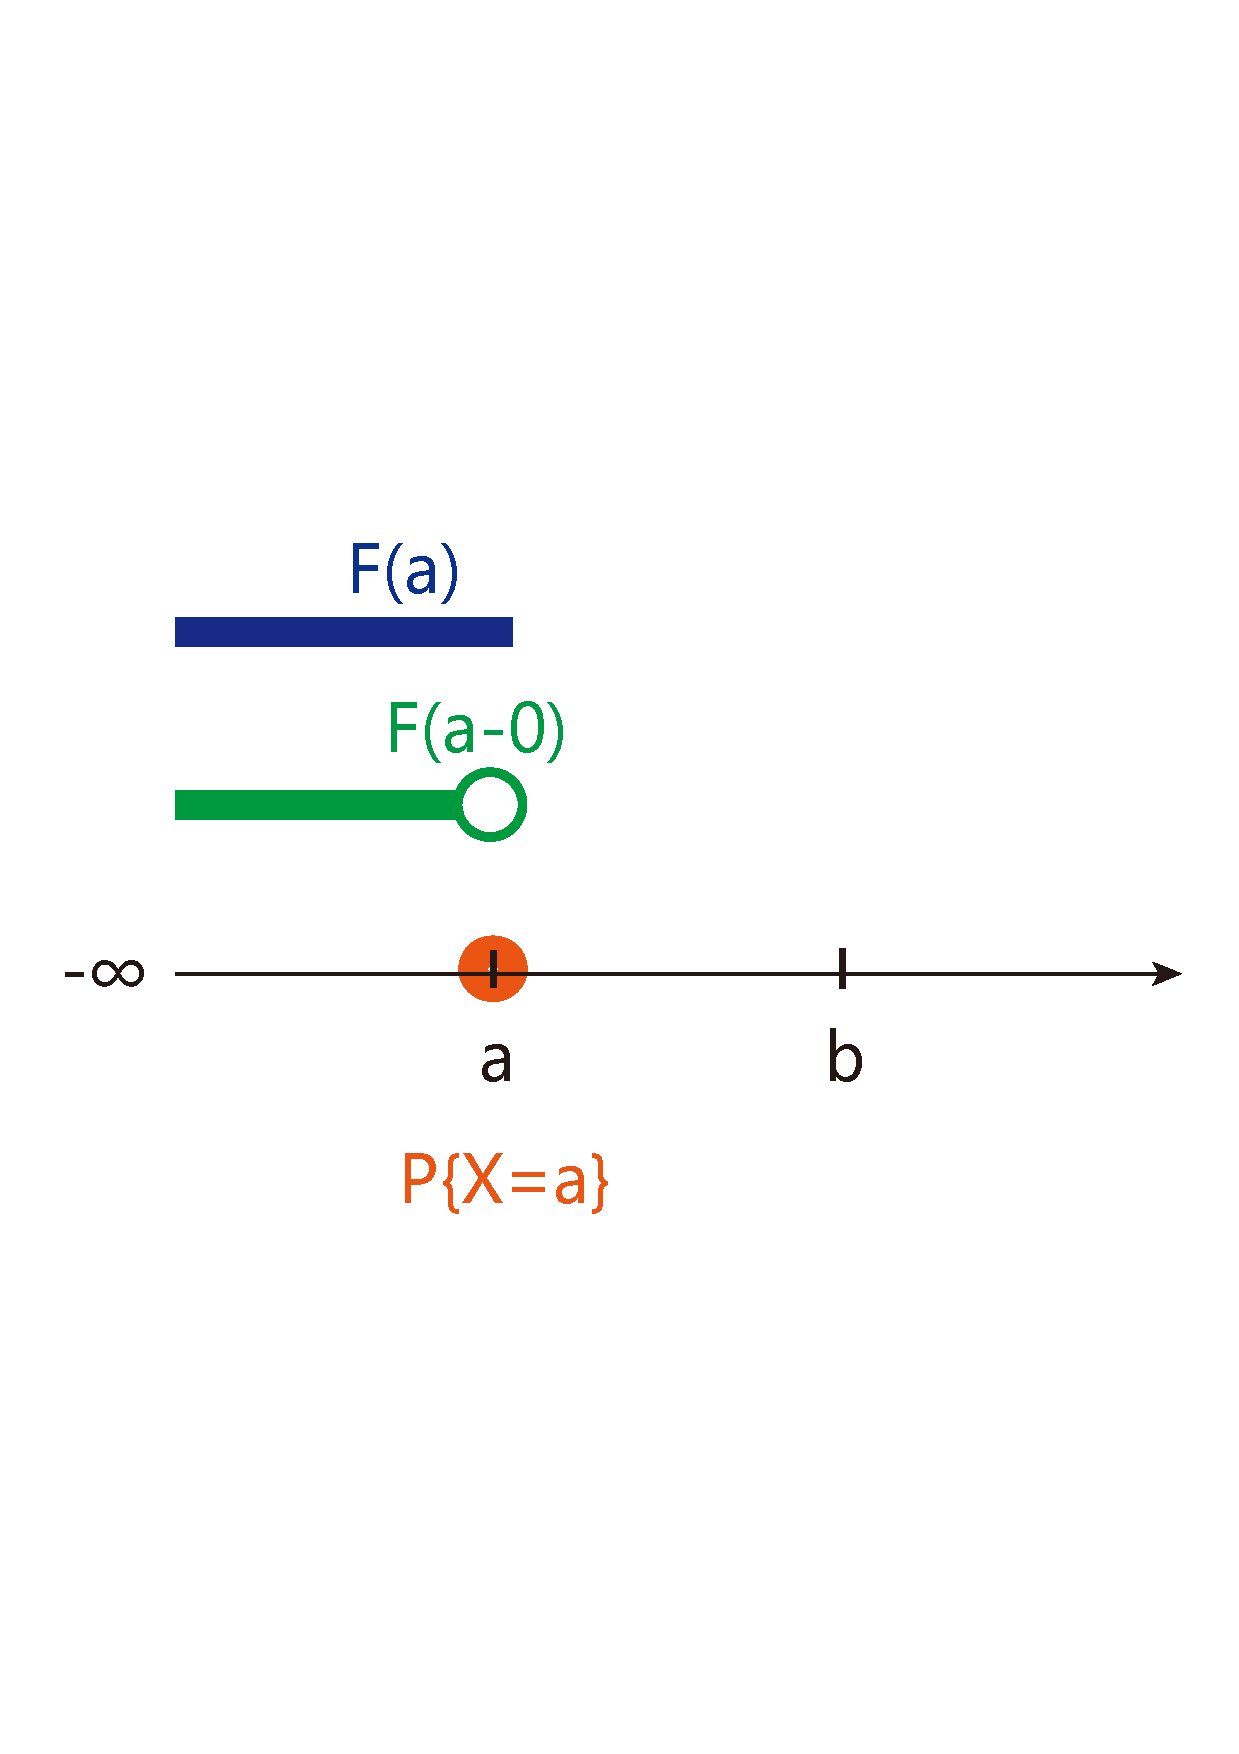
\includegraphics[width=0.35\textwidth]{/0133.pdf}\\ \hline
		(6) $P\{a < X \leq b\} = P(X \leq b) - P(X \leq a)$ &    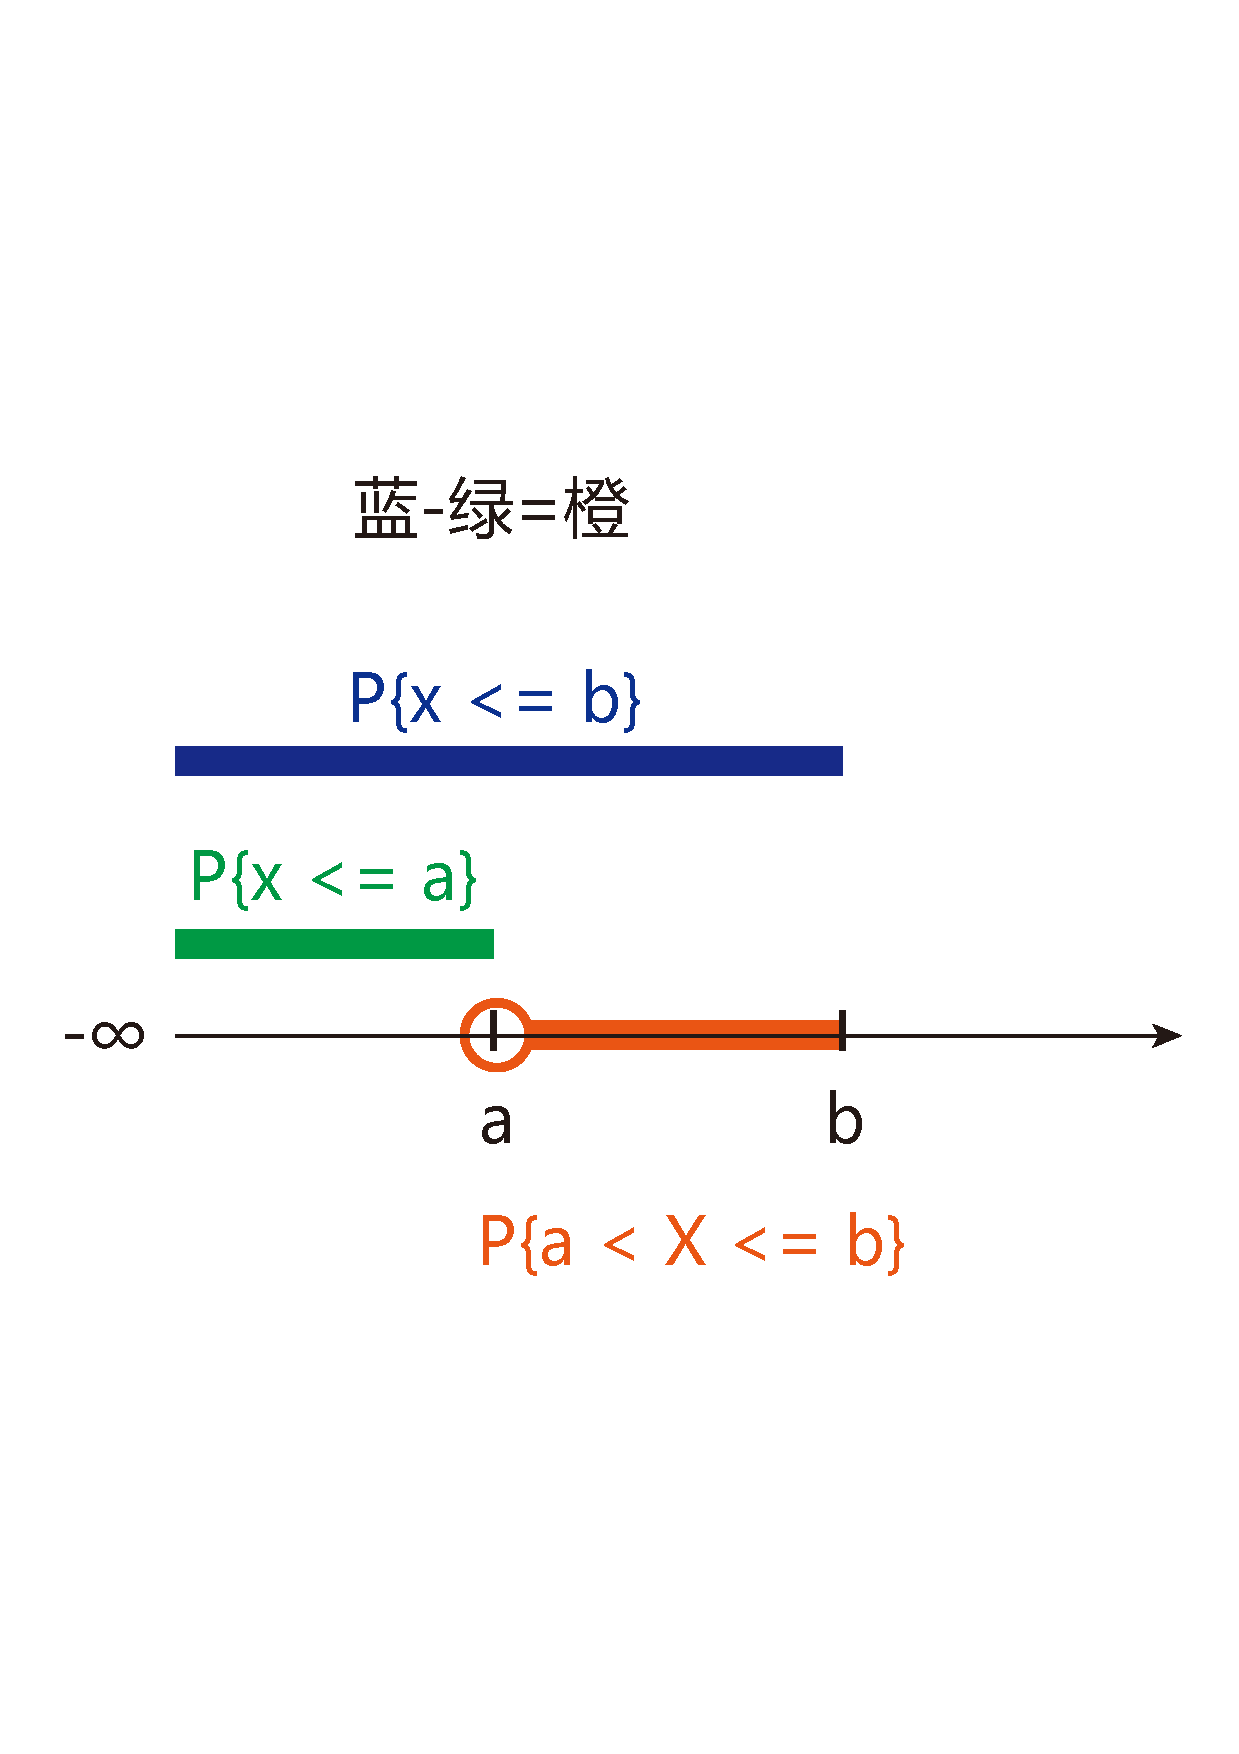
\includegraphics[width=0.35\textwidth]{/0134.pdf}\\ \hline
		(7) $P\{a \leq X \leq b\} = F(b) - F(a-0)$ &   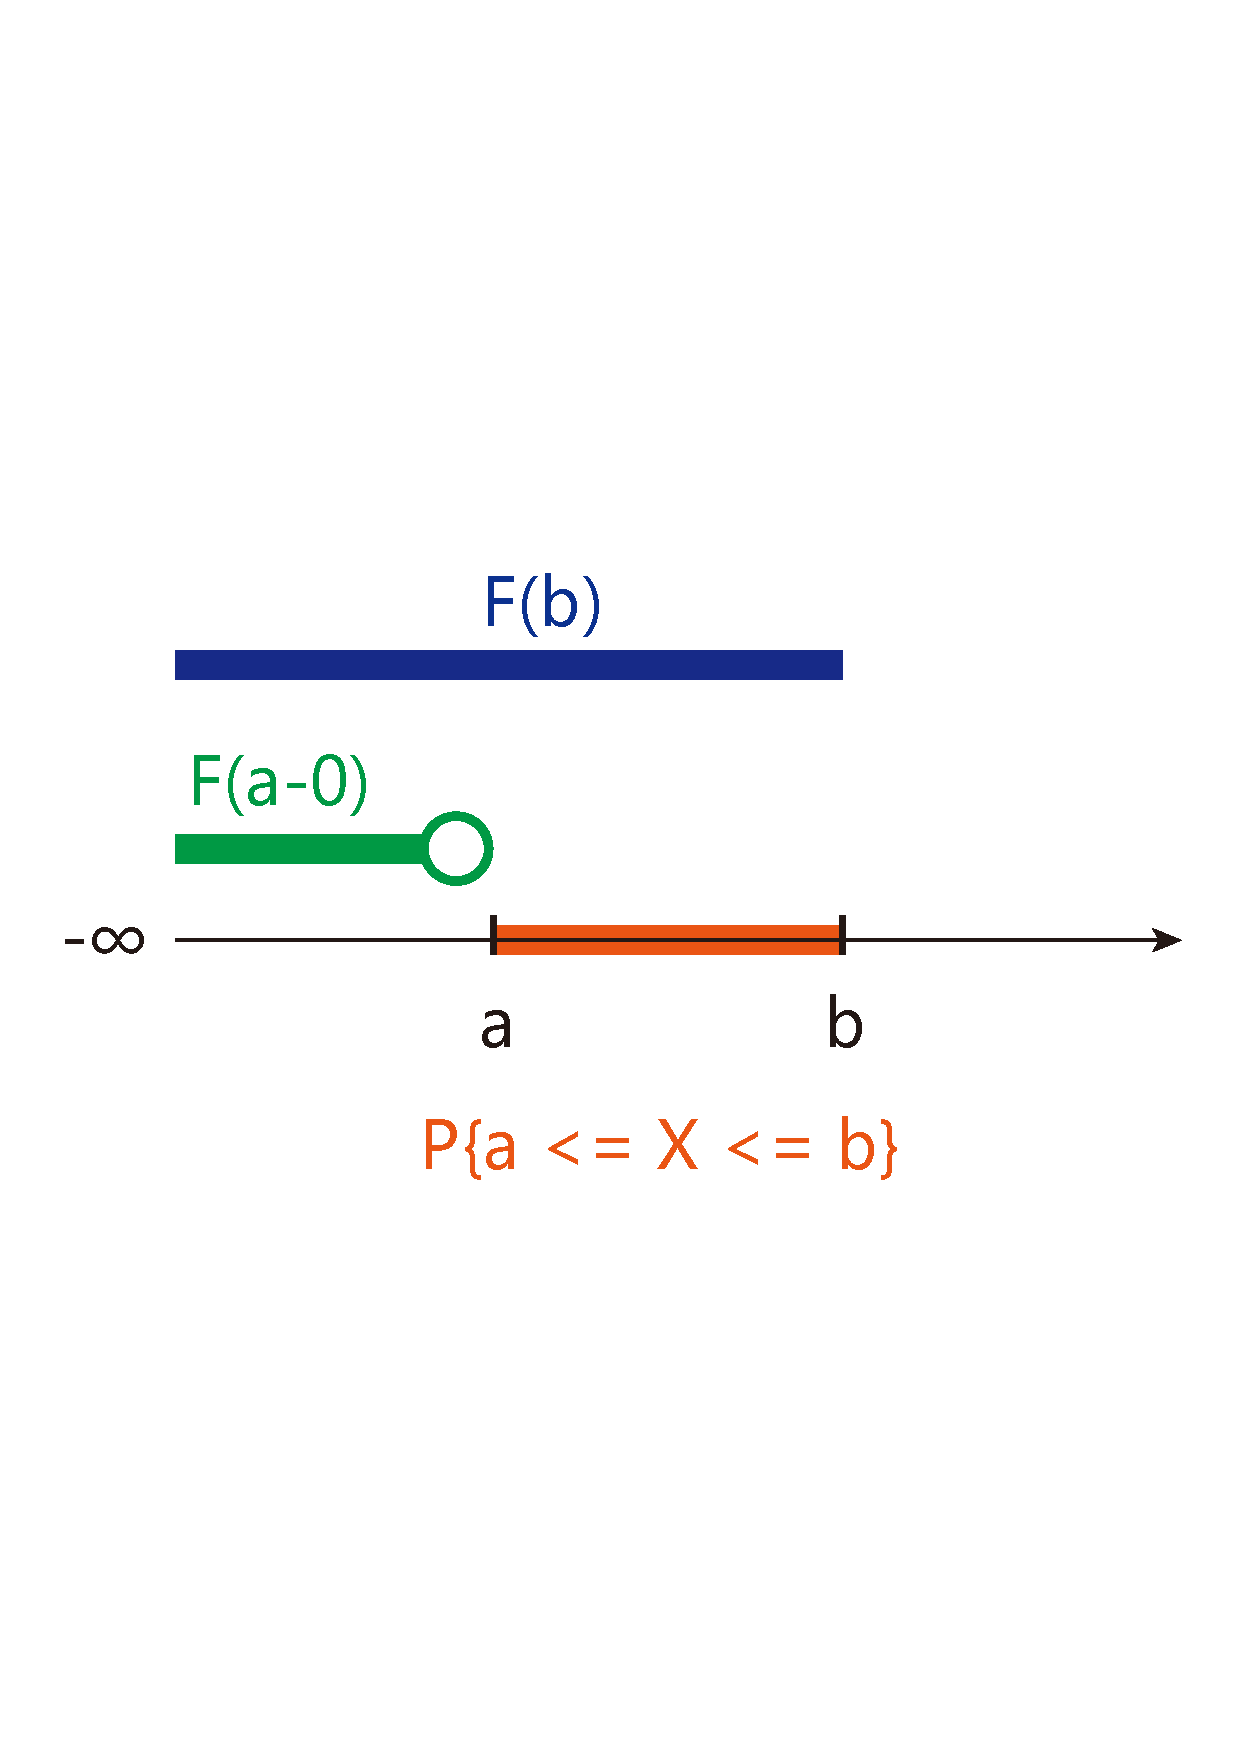
\includegraphics[width=0.35\textwidth]{/0135.pdf} \\ \hline
	\end{tabular}
	
	
	~\\
	\hrule
	~\\
	
	
	
	\section{ 对``概率函数f(x)"求积分, 就得到``累加函数F(x)". 反之, 对``累加函数F(x)"求导, 就得到``概率函数f(x)". 即: \textcircled{1}  $\int_{}^{}{\text{概率函数}f\left( x \right)}=\text{累加函数}F\left( x \right) $, \textcircled{2}
		$\left( \text{累加函数}F\left( x \right) \right) '=\text{概率函数}f\left( x \right) $}
	
	对``概率函数f(x)"求积分, 就得到``累加函数 F(x)" \\
	对``累加函数 F(x)" 求导, 就得到``概率函数f(x)". \\
	
	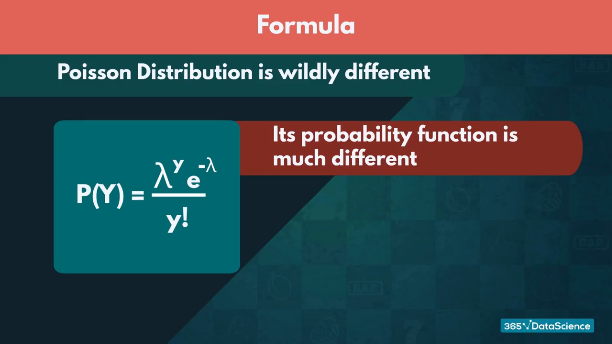
\includegraphics[width=0.8\textwidth]{/0124.png} \\
	
	
	
	\begin{myEnvSample}
		\begin{align*}  % 支持每行编号. 若不需要编号, 就用 align*环境
			&\underset{\text{概率函数}\left( \text{相当于导函数} \right)}{\underbrace{f\left( x \right) }}=\frac{1}{\pi \left( 1+x^2 \right)}\\
			&\underset{\text{累加函数}}{\underbrace{F\left( x \right) }}
			=\int_{-\infty}^x{\underset{\text{概率函数}}{\underbrace{f\left( t \right) }}}dt
			=\int_{-\infty}^x{\underset{\text{导函数}}{\underbrace{\frac{1}{\pi \left( 1+t^2 \right)}}}}dt
			=\frac{1}{\pi}\left( \arctan \mid_{-\infty}^{x} \right) 
			=\frac{1}{\pi}\arctan x+\frac{1}{2}
		\end{align*}
		
		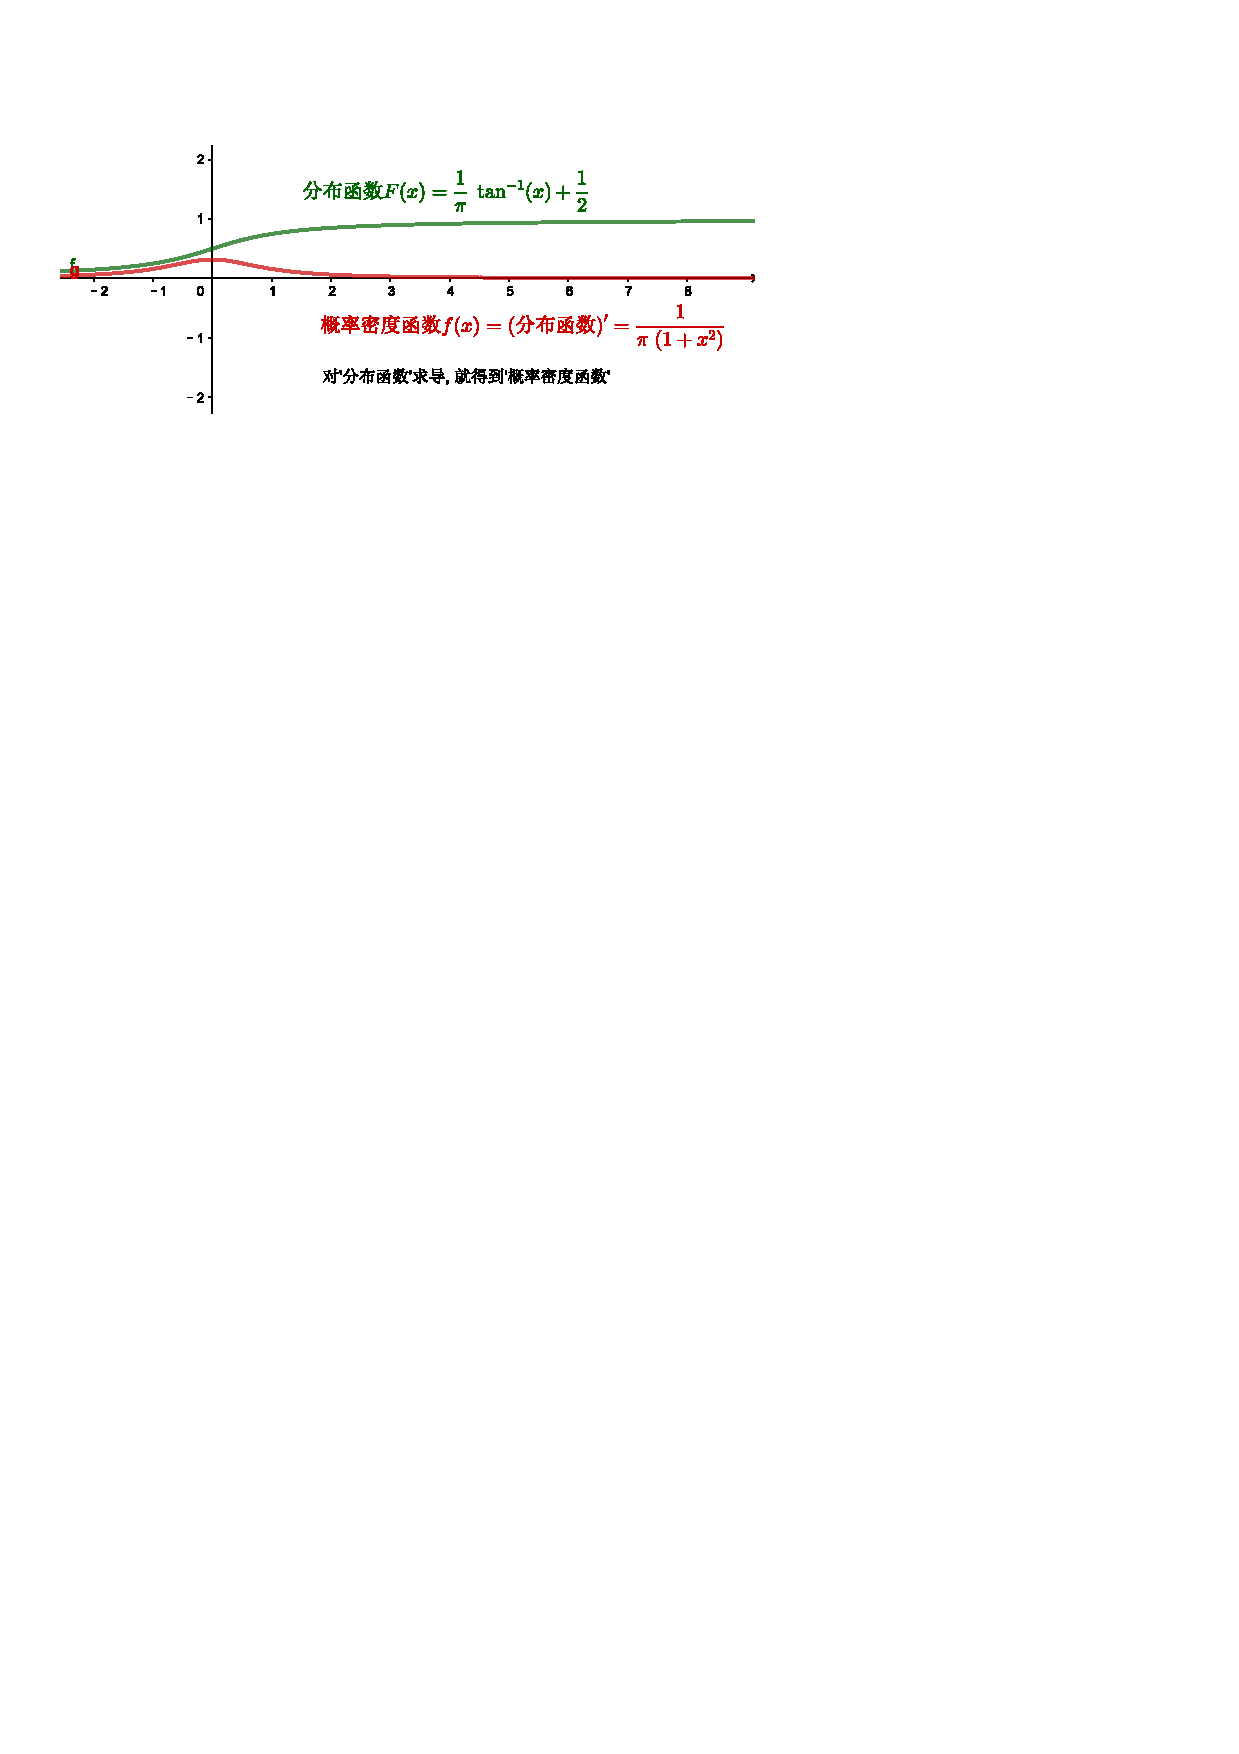
\includegraphics[width=0.7\textwidth]{/0136.pdf}
	\end{myEnvSample}
	\vspace{1em} 
	
	
	
	\begin{myEnvSample}
		有累加函数 $F\left( x \right) =\left\{ \begin{array}{l}
			0\ \ \ \ \ \left( x<0 \right)\\
			Ax^2\ \ \left( 0\leq x<1 \right)\\
			1\ \ \ \ \ \ \left( x\geq 1 \right)\\
		\end{array} \right. $ \\
		
		→ 求常数A :  
		$
		\underset{\text{从}x=1\text{的左侧,逼近}x=1}{\underbrace{\lim_{x\rightarrow 1^-}Ax^2}}=A\left( 1 \right) ^2=A=\underset{\text{因为当}x\geq 1\text{时,}F\left( x \right) =1}{\underbrace{F\left( 1 \right) =1}}
		$ \\
		
		→ 求概率函数f(x) : 
		$
		f\left( x \right) =F'\left( x \right) =\left\{ \begin{array}{l}
			0'=0\ \ \ \ \ \ \ \ \ \ \ \ \ \ \ \ \ \ \left( x<0 \right)\\
			\left( Ax^2 \right) '=\left( x^2 \right) '=2x\ \ \left( 0\leq x<1 \right)\\
			1'=0\ \ \ \ \ \ \ \ \ \ \ \ \ \ \ \ \ \ \left( x\geq 1 \right)\\
		\end{array} \right. 
		$ \\
		
		→ 求 :
		\begin{align*}  % 支持每行编号. 若不需要编号, 就用 align*环境
			&P\left\{ 0.3<X<0.7 \right\} =\underset{=\int_{-\infty}^{0.7}{f\left( t \right)}dt}{\underbrace{F\left( 0.7 \right) }}-\underset{=\int_{-\infty}^{0.3}{f\left( t \right)}dt}{\underbrace{F\left( 0.3 \right) }}\\
			&\text{因为在}0\leq x<1\text{的区间上,}F\left( x \right) =Ax^2,\text{而其中的}A\text{我们上面已经算出}=1,\\
			&\text{所以}F\left( x \right) =Ax^2=\left( 1 \right) x^2=x^2\\
			&\text{所以:\ }F\left( 0.7 \right) =\left( 0.7 \right) ^2=0.49\\
			&F\left( 0.3 \right) =\left( 0.3 \right) ^2=0.09\\
			&\text{因此:\ }P\left\{ 0.3<X<0.7 \right\} =F\left( 0.7 \right) -F\left( 0.3 \right) =0.49-0.09=0.4\\
			&\text{事实上,本例的\ }P\left\{ 0.3<X<0.7 \right\} =\int_{0.3}^{0.7}{\underset{\text{即概率函数}f\left( x \right)}{\underbrace{\left( 2x \right) }}}dx  
		\end{align*}
		
		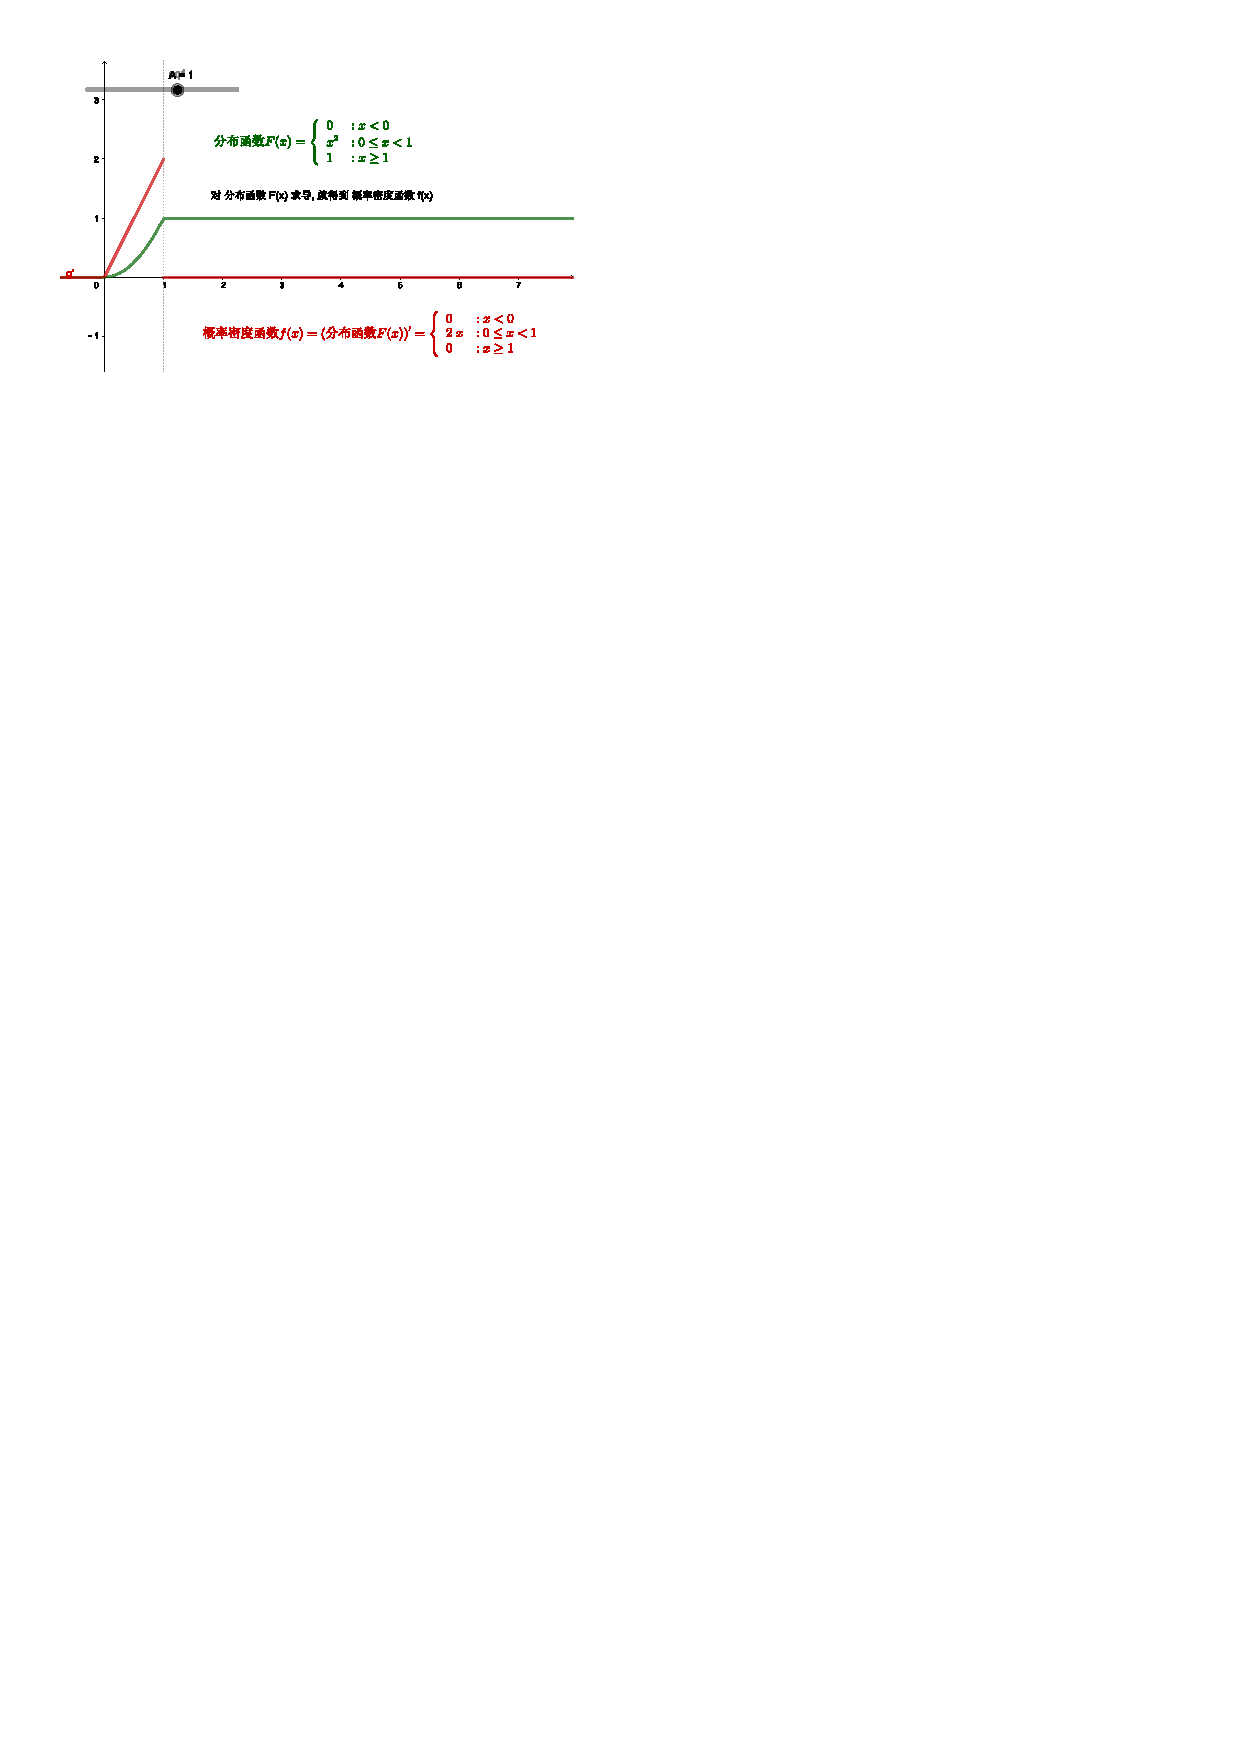
\includegraphics[width=1\textwidth]{/0137.pdf}
		
	\end{myEnvSample}
	
	
	~\\
	\hrule
	~\\
	
	\section{性质}
	
	
	\subsection{性质1: 有界性. $	F\left( x \right) =P\left\{ \text{随机变量}X\leq \text{随机变量的取值}x \right\} ,\ x\in \left( -\infty ,+\infty \right) .\ \text{即\ }0\leq F\left( x \right) \leq 1	$}
	
	累加函数(CDF) F(x), 就是一个普通的实函数. 其定义域是 $x \in (-\infty, +\infty)$. 值域是 $y \in [0,1]$. \\
	
	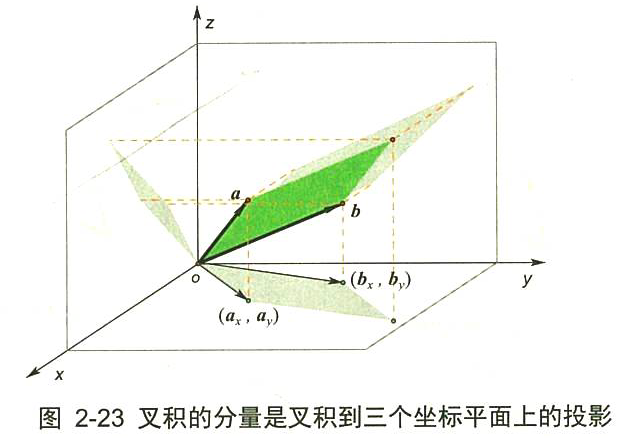
\includegraphics[width=0.5\textwidth]{/0131.png} \\
	
	
	
	累加函数 : \\
	$ \boxed{
		F(x)=P(X\leq a)=\int_{lower\lim it}^a{f\left( x \right) dx}	}$ \\
	\\
	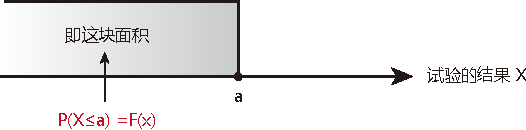
\includegraphics[width=0.6\textwidth]{/0119.pdf} \\
	
	
	$ \boxed{
		P(a\leq X\leq b)=P(a<X<b)=\int_a^b{f\left( x \right) dx}=F\left( b \right) -F\left( a \right) 	} $ \\
	\\
	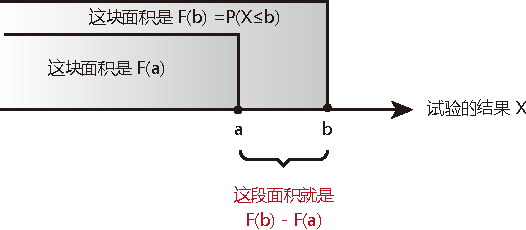
\includegraphics[width=0.6\textwidth]{/0120.pdf} 
	
	
	\begin{align*}  % 支持每行编号. 若不需要编号, 就用 align*环境
		& P(x_1<X\leq x_2)\ ←\ \text{对于随机变量}X\text{在}(x_1,x_2]\text{这段区间上的概率,它的值}\\
		& =F(x_2)-F(x_1)\\
		& =P\{X\leq x_2\}-P\{X\leq x_1\}
	\end{align*} \\
	
	
	对于``连续型随机变量", 有没有两端的端点, 无所谓, 不影响概率值(因为它在任何一个``确定点"的概率都是0嘛). 即: 
	\begin{align*}
		& P \{ a \leq X \leq b \} \\
		& = P \{ a < X \leq b \}  \quad  \text{← 即, 两端是否有``等于号", 无所谓.} \\
		& = P \{ a \leq X < b \}  \\
		& = P \{ a < X < b \}
	\end{align*} 
	
	同样: \\
	$P\{X<a\} = P \{X \leq a \}$  ← 有没有``等于号"无所谓 \\
	$P\{X > a\} = P \{X \geq a \} $
	
	
	
	
	
	\subsection{性质2: 单调不减性. 即 对于任意的 $x_1 < x_2$, 有: $F(x_1) \leq F(x_2)$}
	
	F(x)是关于x的``不减函数", 类似于``单调递增"的概念. ``不减"的意思就是, 该函数的y值不会下降, 只会``增长"或``平移向前". \\
	
	比如, ``分数小于等于70分的人" 其概率一定是小于等于 ``分数小于80分的人". 即 $F(70) \leq F(80)$.
	
	
	
	\subsection{性质3: 规范性. F(-∞)=0 , F(+∞)=1}
	
	$ \boxed{
		\underset{=P(X\leq -\infty )}{\underbrace{F(-\infty )}}=\lim_{x\rightarrow -\infty}F(x)=P(X < - \infty) = P(\Phi)=0
	}$ ← 称之为 ``不可能事件". \\
	如果随机变量X的取值, 比 -∞ 还小, 那其概率, 就只能是0了. \\
	
	
	$\boxed{
		\underset{=P(X\leq +\infty )}{\underbrace{F(+\infty )}}=\lim_{x\rightarrow +\infty}F(x)=P(X < + \infty) = P(\Omega)=1
	}$ ← 称之为 ``必然事件". \\
	如果随机变量X的取值, 在 +∞ 以下, 那其概率, 肯定就是100\%了, 就是1. \\
	
	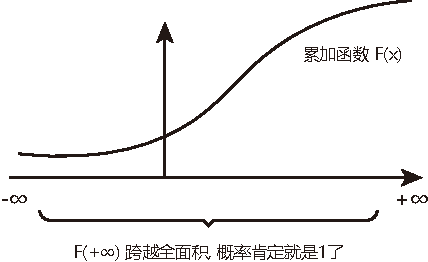
\includegraphics[width=0.5\textwidth]{/0121.pdf} \\
	
	
	
	
	
	
	
	\subsection{性质4 : 右连续性. $\lim_{x \to x_0^+} F(x)=F(x_0)$ }
	
	这个等式的意思就是说: 累加函数在$x_0$点的右极限, 就等于累加函数在该点处的函数值. \\
	
	\begin{tabular}{|p{0.1\textwidth}|p{0.9\textwidth}|}
		\hline
		右连续 &  所谓``右连续", 就是``函数从x在某点的右侧, 逼近该点"的极限值, 就等于``该点处的y值", 即: $\lim_{x \to a^+} F(x) = F(a)$.\\
		\hline
		左连续 &  同理, ``左连续"就是: $\lim_{x \to a^-} F(x) = F(a)$.\\
		\hline
		连续 & 同时满足``左连续"和``右连续"的函数, 就称为是``连续"的. 即 $\lim_{x \to a} F(x) = F(a)$. \\
		\hline
	\end{tabular} \\
	
	满足上面4条性质的, 就一定是``累加函数". 反之, ``累加函数"也一定有这4条性质. \\	
	
	
	
	
	
	
	
\end{document}